\documentclass[../main.tex]{subfiles}

\begin{document}
    \section{Tangent Spaces}
    \begin{remark}
        The definition of manifold do not require the entity to be embeded in 
        a higher dimensional space. Therefore, the traditional view of tangency 
        is not valid here.
        
    \end{remark}

    \subsection{Curves and Vectors}
    \begin{definition}[Curve]\label{def:curve}
        A curve on \(\manifold[M]\) is a \(C^\infty\) map,
        \[
        \sigma : (-\epsilon, \epsilon) \to \manifold[M].
        \]
    \end{definition}
    \begin{definition}[Curve Tangency]\label{def:curve-tangency}
        Two curves \(\sigma_1, \sigma_2\) are tangent at \(p \in \manifold[M]\) 
        if 
        \begin{enumerate}
            \item \(\sigma_1(0)=\sigma_2(0)=p\).
            \item \(\left.\frac{d}{dt}(x^i \circ \sigma_1(t))\right|_{t=0}
             = \left.\frac{d}{dt}(x^i \circ \sigma_2(t))\right|_{t=0},~1 \leq 
             i \leq m\) .
        \end{enumerate}
    \end{definition}
    \begin{remark}
        Written more compactly, 
        \[
        \left.\frac{d}{dt}(\phi\circ\sigma_1)\right|_{t=0}
        =\left.\frac{d}{dt}(\phi\circ\sigma_2)\right|_{t=0}
        \]
        
    \end{remark}
    \begin{definition}[Tangent Vectors]\label{def:tangent-vector-curve}
        A tangent vector at \(p \in \manifold[M]\) is an equivalence class of 
        curves where the equivalence relation is that they are tangent. It will 
        be denoted as 
        \[
        v = [\sigma].
        \]
    \end{definition}
    \begin{definition}[Tangent Space]\label{def:tangent-space-curve}
        The tangent space \(T_p\manifold[M]\) at point \(p\) is the set of all 
        tangent vectors at point \(p\).
    \end{definition}
    
    % \subsection{Addition and Scalar Multiplication}
    % \begin{definition}[Addition and Scalar Multiplication]\label{def:addition-and-scalar-multiplication-curve}
    %     Let \(v_1 = [\sigma_1], v_2 = [\sigma_2] \in T_p\manifold[M]\), and 
    %     \(r \in \mathbb{R}\). Then 
    %     define 
    %     \[
    %     \begin{aligned}
    %         v_1+v_2 &:= [\phi ^{-1}\circ(\phi\circ\sigma_1+\phi\circ\sigma_2)], \\
    %         rv_1 &:= [\phi ^{-1} \circ (r\phi \circ \sigma_1)].
    %     \end{aligned}
    %     \]
    % \end{definition}
    % \begin{theorem}
    %     The definition \cref{def:addition-and-scalar-multiplication-curve}
    %     is well-defined. That is, they are independent of the 
    %     choice of chart \((U, \phi)\) and \(\sigma_1, \sigma_2\) as long as 
    %     \(v_1=[\sigma_1]\) and \(v_2=[\sigma_2]\).\par
    %     Therefore, \(T_p\manifold[M]\) is a real vector space.
    % \end{theorem}
    % \begin{proof}
    %     Let \(v_1 = [\sigma_1] = v_1' := [\tau_1], 
    %     v_2 = [\sigma_2] = v_2' := [\tau_2]\). 
    %     First check (1) of \cref{def:curve-tangency}, 
    %     \[
    %     \begin{aligned}
    %         (rv_1+v_2)(0) &= (\phi ^{-1} \circ (r\phi\circ\sigma_1(0) + 
    %         \phi\circ\sigma_2(0))) \\
    %         &= (\phi ^{-1} \circ (r\phi\circ\tau_1(0) + 
    %         \phi\circ\tau_2(0))) \\
    %         &= (rv_1'+v_2')(0),
    %     \end{aligned}
    %     \]
    %     since \(\phi\circ\sigma_1(0) = \phi\circ\tau_1(0) = \phi(p)\) by 
    %     equivalence, and the same for \(\sigma_2\). \par
    %     Now consider 
    %     \[
    %     \begin{aligned}
    %         \left.\frac{d}{dt}(\phi\circ(rv_1+v_2))\right|_{t=0}
    %         &=\left.\frac{d}{dt}(r\phi\circ\sigma_1+\phi\circ\sigma_2)
    %         \right|_{t=0}\\
    %         &=r\left.\frac{d}{dt}(\phi\circ\sigma_1)\right|_{t=0}+
    %         \left.\frac{d}{dt}(\phi\circ\sigma_2)\right|_{t=0}\\
    %         &=r\left.\frac{d}{dt}(\phi\circ\tau_1)\right|_{t=0}+
    %         \left.\frac{d}{dt}(\phi\circ\tau_2)\right|_{t=0}\\
    %         &=\left.\frac{d}{dt}(\phi\circ(rv_1'+v_2'))\right|_{t=0},
    %     \end{aligned}
    %     \]
    %     since \(\left.\frac{d}{dt}(\phi\circ\sigma_1)\right|_{t=0}
    %     =\left.\frac{d}{dt}(\phi\circ\tau_1)\right|_{t=0}\) by equivalence, and 
    %     the same for \(\sigma_2\).
    % \end{proof}

    \subsection{Curves and Derivation}
    \begin{definition}[Directional Derivative]\label{def:directional-derivative-curve}
        For any \(f : \manifold[M] \to \mathbb{R}\) s.t. \(f \in C^\infty\), we 
        define
        \[
        v(f) := \left.\frac{d}{dt}(f \circ \sigma(t))\right|_{t=0},
        \]
        where \(v = [\sigma]\).
    \end{definition}
    \begin{theorem}
        The definition \cref{def:directional-derivative-curve} is well-defined.
        That is, \(v(f)\) is independent of the curve \(\sigma\) chosen as well 
        as \(v=[\sigma]\).
    \end{theorem}
    \begin{proof}
        Let \(v_1 = [\sigma_1] = [\sigma_2] = v_2\). Then 
        \[
        \begin{aligned}
            v_1(f) &= \left.\frac{d}{dt}(f \circ \sigma_1)\right|_{t=0}, \\
            v_2(f) &= \left.\frac{d}{dt}(f \circ \sigma_2)\right|_{t=0}, \\
        \end{aligned}
        \]
        \[
        \left.\frac{d}{dt}(\phi\circ\sigma_1)\right|_{t=0}
            =\left.\frac{d}{dt}(\phi\circ\sigma_2)\right|_{t=0}.
        \] \par
        Then
        \[
        \begin{aligned}
            v_1(f) &= \left.\frac{d}{dt}
            (\underbrace{(f\circ\phi ^{-1})}_{\mathbb{R}\leftarrow \mathbb{R}^m} \circ 
            \underbrace{(\phi \circ \sigma_1)}_{\mathbb{R}^m\leftarrow \mathbb{R}})
            \right|_{t=0} \\
            &= \left.(f \circ \phi ^{-1})'\circ(\phi\circ\sigma_1)\cdot
            (\phi\circ\sigma_1)'\right|_{t=0} \\
            &= \left.(f \circ \phi ^{-1})'\circ(\phi\circ\sigma_2)\cdot
            (\phi\circ\sigma_2)'\right|_{t=0} \\
            &= v_2(f),
        \end{aligned}
        \]
        since \(\phi\circ\sigma_1(0) = \phi\circ\sigma_2(0) =\phi(p)\), and 
        \((\phi\circ\sigma_1)'=(\phi\circ\sigma_2)'\) by equivalence.
    \end{proof}

    \subsection{Isomorphism with Euclidean Spaces}
    \begin{definition}["Straight Lines"]\label{def:map-straight}
        Choose a coordinate chart \(\phi \in \Phi\) atlas near \(p\). 
        For all \(v \in \mathbb{R}^m\), we define 
        \[
        \gamma_v^\phi(t) := \phi ^{-1}(\phi(p)+tv).
        \]
        In simple words, it is such a curve on manifold that it is a straight line 
        on maps.
    \end{definition}
    \begin{theorem}[Isomorphism with Straight Lines]\label{thm:curve-straight-iso}
        Let \(p \in \manifold[M]\), \(p \in \phi \in \Phi\). For any curve 
        \(\gamma\) passing through \(p\), \(\exists!~v \in \mathbb{R}^m\) s.t. 
        \(\gamma\) is tangent to \(\gamma_v^\phi\), where \(v\) can be explicitly 
        given by \((\phi \circ \gamma)'(0)\). \\
        In other words, the map
        \[
        \begin{aligned}
            \ell_p^\phi : & \mathbb{R}^m \to T_p\manifold[M] \\
                          & v \mapsto [\gamma_v^\phi]
        \end{aligned}
        \]
        is a bijection with inverse 
        \[
        \begin{aligned}
            (\ell_p^\phi) ^{-1} : & T_p\manifold[M] \to \mathbb{R}^m \\
                          & [\gamma] \mapsto (\phi \circ \gamma)'(0).
        \end{aligned}
        \]
    \end{theorem}
    \begin{proof}
        It is almost by definition that \(\gamma\) is tangent to 
        \((\phi \circ \gamma)'(0)\). \par
        Suppose \(v_1, v_2\) satisfies \(\gamma\) is tangent to 
        \(\gamma_{v_1}^\phi, \gamma_{v_2}^\phi\). Then they are tangent too. So 
        \[
        (\phi \circ \gamma_{v_1}^\phi)'(0) = (\phi \circ \gamma_{v_2}^\phi)'(0).
        \]
        Therefore, \(v_1=v_2\).
    \end{proof}
    \begin{definition}[Alternative Definition for Addition]\label{def:curve-add-alt}
        For \(v_1, v_2 \in T_p\manifold[M]\), we define addition via the isomorphism 
        \cref{thm:curve-straight-iso}, 
        \[
        v_1 + v_2 := (\ell_p^\phi)^{-1}(\ell_p^\phi(v_1)+\ell_p^\phi(v_2)).
        \]
    \end{definition}
    \newpage
    \begin{definition}[Alternative Definition of Basis Tangent Vectors]\label{def:basis-alt}
        \[
        \tvec{\mu}{p} := \ell_p^\phi(e^\mu).
        \]
    \end{definition}
    \begin{theorem}
        \[
        \tvec{\mu}{p}(x^\nu) = \delta\indices{_\mu^\nu}.
        \]
    \end{theorem}
    \begin{proof}
        By \cref{def:basis-alt}, 
        \[
        \tvec{\mu}{p} := \ell_p^\phi(e^\mu) = \phi ^{-1}(\phi(p)+te^\mu), 
        \]
        where \(e^\mu\) is the column vector with \(\mu\)-th component 1, others 
        0. Then 
        \[
        \begin{aligned}
            \tvec{\mu}{p}(x^\nu)&=(x^\nu\circ\phi ^{-1}(\phi(p)+te^\mu))'(0) \\
            &=(x^\nu \circ \phi ^{-1})'(\phi(p))e^\mu.
        \end{aligned}
        \]
        But since \(x^\nu\) has only one component, \((x^\nu \circ \phi ^{-1})'\) 
        is a row vector with \(\nu\)-th component 1, others 0. So the result 
        follows immediately.
    \end{proof}
    \begin{theorem}[Linear Independence of Basis Tangent Vectors]\label{thm:linear-indep-basis}
        The basis tangent vectors \(\tvec{\mu}{p}, 1 \leq \mu \leq \dim 
        \manifold[M]\) are linear independent.
    \end{theorem}
    \begin{proof}
        Suppose \(a^\mu\tvec{\mu}{p}=0\). Then 
        \[
        a^\mu\tvec{\mu}{p}(x^\nu)=a^\mu\delta\indices{^\nu_\mu}=0(x^\nu)=0.
        \]
        So \(a^\nu=0\).
    \end{proof}
    \begin{theorem}[Coordinate Expansion of Tangent Vectors]\label{thm:tangent-vector-coordinates}
        For all \(v \in T_p\manifold[M]\), we have 
        \[
        v=v^\mu\tvec{\mu}{p},
        \]
        where Einstein notation was used, and \(v^\mu = v(x^\mu)\).
    \end{theorem}
    \begin{remark}
        A natural question is that whether two charts behave "the same" if 
        \(U_1 \cap U_2 \neq \varnothing\). Under this perspective, the criterion 
        is clear: we need only to check whether a straight line is still a straight 
        line in another chart, which is true indeed. It also produces the coordinate 
        transformation formula for free. See below.
    \end{remark}
    \begin{theorem}[Coordinate Transformation of Straight Lines]\label{thm:straight-overlap}
        Choose \(\phi, \psi \in \Phi\), \(\phi : U_1 \to \mathbb{R}^m\), 
        \(\psi : U_2 \to \mathbb{R}^m\) s.t. \(U_1 \cap U_2 \neq \varnothing\) and 
        \(p \in U_1 \cap U_2\). Let the corresponding straight line isomorphisms 
        \(\ell_p^\phi, \ell_p^\psi\). Then \((\ell_p^\psi)^{-1} \circ \ell_p^\phi\) 
        is a linear isomorphism. \\
        Let the local coordinates induced by \(\phi\) be \(x^1, \dots, x^m\), 
        \(\psi\) be \(y^1, \dots, y^m\), then 
        \((\ell_p^\psi)^{-1} \circ \ell_p^\phi\) can be expressed in terms of 
        the Jacobian \cref{def:jacobian-matrix} \(J\indices{^\nu_\mu}:=
        \left.\frac{\partial y^\nu}{\partial x^\mu}\right|_{\phi(p)}\), namely, 
        \[
        (\ell_p^\psi)^{-1} \circ \ell_p^\phi(v) = Jv.
        \]
    \end{theorem}
    \begin{proof}
        \[
        \begin{aligned}
            (\ell_p^\psi)^{-1} \circ \ell_p^\phi(v) &= 
            (\ell_p^\psi)^{-1}(\phi ^{-1}(\phi(p)+vt)) \\
            &= ((\psi \circ \phi ^{-1})(\phi(p)+vt))'(0) \\
            & = Jv \\
        \end{aligned}
        \]
    \end{proof}
    \begin{definition}[Contravariancy and Covariancy]\label{def:contravariant-covariant}
        Let \(\manifold[M]\) be a \(m\)-dimensional \(C^\infty\) manifold. 
        Choose two coordinate charts
        \[
        \begin{aligned}
            \phi : U_\phi \to V_\phi,& \; p \mapsto (x^1(p), \dots, x^m(p)), \\
            \psi : U_\psi \to V_\psi,& \; p \mapsto (y^1(p), \dots, y^m(p)).
        \end{aligned}
        \]
        and the corresponding Jacobian matrix \cref{def:jacobian-matrix} 
        \(J\indices{^\nu_\mu} := \left.\frac{\partial y^\nu}{\partial x^\mu}
        \right|_{\phi(p)}\).
        We define covariancy to be anything that transforms like 
        \[
        (\text{new})_\nu = (\text{old})_\mu(J^{-1})\indices{^\mu_\nu}.
        \]
    \end{definition}
    \begin{corollary}[Contravariancy of Tangent Vectors]\label{cor:vec-coord-trans}
        The basis vectors transform covariantly, whereas the components of 
        vectors transform contravariantly. That is, choose two overlapping 
        coordinate charts \((x^1, \dots, x^m)\) and \((y^1, \dots, y^m)\) and define 
        their Jacobian matrix \cref{def:jacobian-matrix} \(J\indices{^\nu_\mu} := 
        \left.\frac{\partial y^\nu}{\partial x^\mu}\right|_{\phi(p)}\), 
        \[
        \begin{cases}
            \left(\frac{\partial }{\partial y^\nu}\right) = 
            \left(\frac{\partial }{\partial x^\mu}\right)(J^{-1})\indices{^\mu_\nu}
            & \text{(covariant)} \\
            v^{\nu'} = J\indices{^{\nu'}_\mu}v^\mu & \text{(contravariant)}
        \end{cases}
        \]
    \end{corollary}
    \subsection{Pushforward}
    \subsubsection{Definition and Linearity}
    \begin{remark}
        The pushforward \(h_* : T_p\manifold[M] \to 
        T_{h(p)}\manifold[N]\) of a specific function \(h : \manifold[M] \to 
        \manifold[N]\) can be thought of as local linearization of the function.
        
    \end{remark}
    \begin{definition}[Pushforward]\label{def:pushforward}
        Given a function \(h : \manifold[M] \to \manifold[N]\) and 
        \(v \in T_p\manifold[M]\), then we define the pushforward 
        \(h_* : T_p\manifold[M] \to T_{h(p)}\manifold[N]\) by 
        \[
        h_*(v) := [h \circ \sigma],~v=[\sigma].
        \]
    \end{definition}
    \begin{theorem}
        The pushforward operation \cref{def:pushforward} is well-defined. That is, 
        \(h_*(v_1) = h_*(v_2)\) if \(v_1 = [\sigma_1] = [\sigma_2] = v_2\).
    \end{theorem}
    \begin{theorem}[Algebraic Definition of Pushforward]\label{thm:algebraic-pushforward}
        The definition of pushforward \cref{def:pushforward} is equivalent to the 
        following: let \(h : \manifold[M] \to \manifold[N]\), \(h_* : 
        D_p\manifold[M] \to D_{h(p)}\manifold[M]\) is defined by,
        \[
        (h_*v)(f) := v(f\circ h).
        \]
    \end{theorem}
    \begin{proof}
        (\textrightarrow) 
        \[
        \begin{aligned}
            h_*(v)(f) = [h \circ \sigma](f) 
            &= \left.\frac{d}{dt}(f\circ h\circ\sigma(t))\right|_{t=0} \\
            &= \left.\frac{d}{dt}((f\circ h)\circ\sigma(t))\right|_{t=0} \\
            &:= v(f\circ h).
        \end{aligned}
        \] \par
        (\textleftarrow) This direction is similar.
    \end{proof}
    \begin{theorem}[Linearity of Pushforward]\label{thm:linearity-of-pushforward}
        The pushforward map \(h_* : T_p\manifold[M] \to T_{h(p)}\manifold[N]\) 
        is linear.
        \[
        h_*(rv_1+v_2) = rh_*(v_1) + h_*(v_2).
        \]
    \end{theorem}
    \begin{proof}
        (Using \cref{def:pushforward})
        Let \(p \in (U, \phi) \subseteq \manifold[M]\), and 
        \(h(p) \in (V, \psi) \subseteq \manifold[N]\). Choose \(\phi\) s.t. 
        \(\phi(p) = 0\).
        It is obvious that \(h_*(rv_1+v_2)(0) = (rh_*(v_1)+h_*(v_2))(0) = h(p)\). 
        \par
        Consider 
        \[
        \begin{aligned}
            \left.\frac{d}{dt}
            \underbrace{(\psi \circ h_*(rv_1+v_2))}_{\mathbb{R}^n \leftarrow 
            \manifold[N] \leftarrow \mathbb{R}}\right|_{t=0}
            &= \left.\frac{d}{dt}(\underbrace{\psi\circ h\circ (\phi ^{-1}}
            _{\mathbb{R}^n \leftarrow \manifold[N] \leftarrow \manifold[M] 
            \leftarrow \mathbb{R}^m}\circ
            \underbrace{(r\phi\circ\sigma_1+\phi\circ\sigma_2)}_{\mathbb{R}^m 
            \leftarrow \manifold[M] \leftarrow \mathbb{R}}))\right|_{t=0} \\
            &= \left.(\psi \circ h \circ \phi ^{-1})'\circ 
            (r\phi\circ\sigma_1+\phi\circ\sigma_2) \cdot (r\phi\circ\sigma_1 + 
            \phi\circ\sigma_2)'\right|_{t=0} \\
            &= \left.(\psi \circ h \circ \phi ^{-1})'(0) \cdot 
            ((r\phi\circ\sigma_1)' + (\phi\circ\sigma_2)')\right|_{t=0}.
        \end{aligned}
        \]
        And 
        \[
        \begin{aligned}
            \left.\frac{d}{dt}
            (\underbrace{\psi}_{\mathbb{R}^n\leftarrow} \circ 
            \underbrace{(rh_*(v_1)+h_*(v_2))}_{\manifold[N]\leftarrow 
            \mathbb{R}})
            \right|_{t=0}
            &= \left.\frac{d}{dt}
            \underbrace{(r\psi\circ h \circ \sigma_1 + \psi \circ h \circ \sigma_2)}_
            {\mathbb{R}^n \leftarrow \manifold[N] \leftarrow \manifold[M] \leftarrow 
            \mathbb{R}}
            \right|_{t=0} \\
        \end{aligned}
        \]
        \[
        \begin{aligned}
        =&(\underbrace{r\psi\circ h\circ \phi ^{-1}}_
        {\mathbb{R}^n\leftarrow\manifold[N]\leftarrow\manifold[M]
        \leftarrow\mathbb{R}^m} \circ \underbrace{\phi \circ \sigma_1}_
        {\mathbb{R}^m\leftarrow\manifold[M]\leftarrow\mathbb{R}} + 
        \psi\circ h\circ \phi ^{-1} \circ \phi \circ \sigma_2
        )'|_{t=0} \\
        =&(r(\psi\circ h\circ \phi ^{-1})'\circ(\phi\circ\sigma_1)
        \cdot(\phi\circ\sigma_1)')|_{t=0} \\
        &+((\psi\circ h\circ \phi ^{-1})'\circ(\phi\circ\sigma_2)
        \cdot(\phi\circ\sigma_2)')|_{t=0} \\
        =&(\psi\circ h\circ \phi ^{-1})'(0)\cdot(r(\phi\circ\sigma_1)' + 
        (\phi\circ\sigma_2)')|_{t=0}.
        \end{aligned}
        \]
        So we see the two are equal. \par
        (Using \cref{thm:algebraic-pushforward})
        \[
        \begin{aligned}
            (h_*(rv_1+v_2))(f) &= (rv_1+v_2)(f\circ h) \\
            &= rv_1(f\circ h)+v_2(f\circ h) \\
            &= r(h_*v_1)f+(h_*v_2)f.
        \end{aligned}
        \]
        \par
        (Using straight line isomorphism: \cref{def:curve-add-alt})
        \begin{center}
            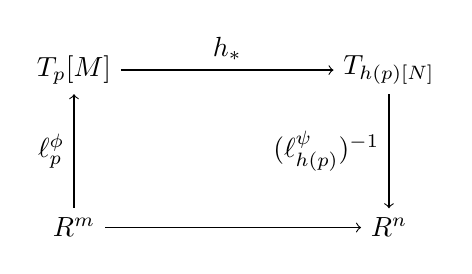
\begin{tikzpicture}
    \node (tpm) at (0, 0) {$T_p\manifold[M]$};
    \node (thpn) at (4, 0) {$T_{h(p)\manifold[N]}$};
    \node (rm) at (0, -2) {$\mathbb{R}^m$};
    \node (rn) at (4, -2) {$\mathbb{R}^n$}
        edge[<-] (rm);
    \draw[->] (tpm.east) -- (thpn.west) node[midway, above] {$h_*$};
    \draw[<-] (tpm.south) -- (rm.north) node[midway, left] {$\ell_p^\phi$};
    \draw[->] (thpn.south) -- (rn.north) node[midway, left] 
        {$(\ell_{h(p)}^\psi)^{-1}$};
\end{tikzpicture}
        \end{center}
        Since \(\ell_p^\phi\) and \((\ell_{h(p)}^\psi)^{-1}\) are linear, to prove 
        \(h_*\) is linear, we need only to show \((\ell_{h(p)}^\psi)^{-1} \circ 
        h_* \circ \ell_p^\phi\) is linear. \par
        \[
        \begin{aligned}
            &(\ell_{h(p)}^\psi) ^{-1} \circ h_* \circ \ell_p^\phi(v) \\
            =&(\ell_{h(p)}^\psi)^{-1} \circ h_*([\phi ^{-1}(\phi(p)+tv)]) \\
            =&(\ell_{h(p)}^\psi)^{-1}([h\circ\phi ^{-1}(\phi(p)+tv)]) \\
            =&(\psi \circ h \circ \phi ^{-1}(\phi(p)+tv))'(0) \\
            =&(\psi \circ h \circ \phi ^{-1})'(\phi(p))v.
        \end{aligned}
        \]
    \end{proof}
    \begin{theorem}[Associativity of Pushforwards]\label{thm:pushforward-associativity}
        Given manifolds \(\manifold[M], \manifold[N], \manifold[P]\) and 
        \(h : \manifold[M] \to \manifold[N]\), \(k : \manifold[N] \to 
        \manifold[P]\), then 
        \[
        (k\circ h)_*=k_*\circ h_*.
        \]
    \end{theorem}

    \subsubsection{Jacobian}
    \begin{theorem}[Local Representative of Pushforward]\label{thm:pushforward-local}
        Let \(\dim \manifold[M]=m, \dim \manifold[N]=n\), \(h : \manifold[M] 
        \to \manifold[N]\), \(\{x^1, \dots, x^m\}\) be the local coordinates of 
        \(\manifold[M]\) around \(p\), and \(\{y^1, \dots, y^n\}\) be the local 
        coordinates of \(\manifold[N]\) around \(h(p)\). Then 
        \[
        h_*v = \sum_{\mu=1}^{m} \sum_{\nu=1}^{n} \tvec{\nu}{h(p)} 
        \left.\frac{\partial h^\nu}{\partial x^\mu}\right|_{p}v^\mu,
        \]
        where \(J\indices{^\nu_\mu}:=\left.\frac{\partial h^\nu}{\partial x^\mu}\right|_{p}
        :=\tvec{\mu}{p}(y^\nu\circ h)\) is the Jacobian matrix.
    \end{theorem}
    \begin{proof}
        First expand \(v\) in terms of local coordinates and use linearity, 
        \[
        h_*v = h_*(v^\mu \tvec{\mu}{p}) = v^\mu h_*(\tvec{\mu}{p}).
        \]
        Expand the result in local coordinates of \(\manifold[N]\), 
        \[
        h_*(\tvec{\mu}{p}) = \left(h_*\tvec{\mu}{p}\right)^\nu\tvec{\nu}{h(p)}.
        \]
        Using \cref{thm:algebraic-pushforward}, 
        \[
        \begin{aligned}
            \left(h_*\tvec{\mu}{p}\right)^\nu 
            &= \left(h_*\tvec{\mu}{p}\right)\circ y^\nu \\
            &= \tvec{\mu}{p}(y^\nu \circ h) \\
            &:= \tvec{\mu}{p}h^\nu.
        \end{aligned}
        \]
        So, 
        \[
        h_*(\tvec{\mu}{p}) = \tvec{\mu}{p}h^\nu\tvec{\nu}{h(p)}.
        \]
        And, 
        \[
        h_*v = v^\mu\tvec{\mu}{p}h^\nu\tvec{\nu}{h(p)}.
        \]
    \end{proof}
    \begin{theorem}[Using Curve to Pushforward]\label{thm:curve-pushforward}
        Given \(c : (-\epsilon, \epsilon) \to \manifold[M]\) a curve, and choose 
        the coordinate chart of \(\mathbb{R}\) to be the identity, then 
        \[
        c_*\left(\frac{d}{dt}\right)_0=[c] \in T_p\manifold[M].
        \]
    \end{theorem}
    \begin{proof}
        First we clarify what is \(\left(\frac{d}{dt}\right)_0\). Since on the 
        trivial manifold \(\mathbb{R}\) there is only one coordinate, namely 
        \(t\), we need not specify the number. Also, considering our functions 
        are scalar valued \(f : \manifold[M] \to \mathbb{R}\), this motivates us 
        to write "total differential". \par
        For all \(f \in C^\infty\), 
        \[
        c_*\left(\frac{d}{dt}\right)_0f=\left(\frac{d}{dt}\right)_0(f\circ c).
        \]
        Since the coordinate chart is the identity, 
        \[
        \begin{aligned}
            \left(\frac{d}{dt}\right)_0(f\circ c) 
            &= \left.\frac{d}{dt}(f\circ c\circ I)\right|_{I(t)=0} \\
            &= \left.\frac{d}{dt}(f\circ c)\right|_{t=0} \\
            &=[c]f.
        \end{aligned}
        \]
    \end{proof}
\end{document}